\section{Evaluation}

\subsection{Evaluate Results}

CRISP-DM separates model assessment from evaluation. The Modeling stage showed that XGBoost with diff embeddings is the best candidate technically. The Evaluation stage asks a broader question: whether the model and the other findings answer the original business problem.

The result is partially successful. The dataset objective is satisfied: the project produced 10,000 enriched pull request workflows, of which 7,373 pass the current quality filters, across 6,033 repositories. This is above the target of 5,000 curated workflows and supports the business objective of creating a reusable workflow dataset. The downstream modeling goal is also satisfied at baseline level: the selected model reaches ROC-AUC 0.628 against random 0.500, and macro-F1 0.537 against the majority-class baseline of 0.490.

\begin{table}[H]
\centering
\small
\begin{tabular}{p{0.29\linewidth}p{0.22\linewidth}p{0.18\linewidth}p{0.11\linewidth}}
\hline
Criterion & Target & Measured & Verdict \\
\hline
Curated workflow volume & At least 5,000 accepted rows & 7,373 & Pass \\
Repository coverage & Multi-repository dataset & 6,033 repositories & Pass \\
Ranking signal & ROC-AUC above 0.500 & 0.628 & Pass \\
Baseline improvement & Macro-F1 above 0.490 & 0.537 & Pass \\
Demonstrable artifact & Dataset and demo application & Dataset page and local demo & Pass \\
\hline
\end{tabular}
\caption{Evaluation scorecard against the project success criteria.}
\end{table}

\begin{figure}[H]
    \centering
    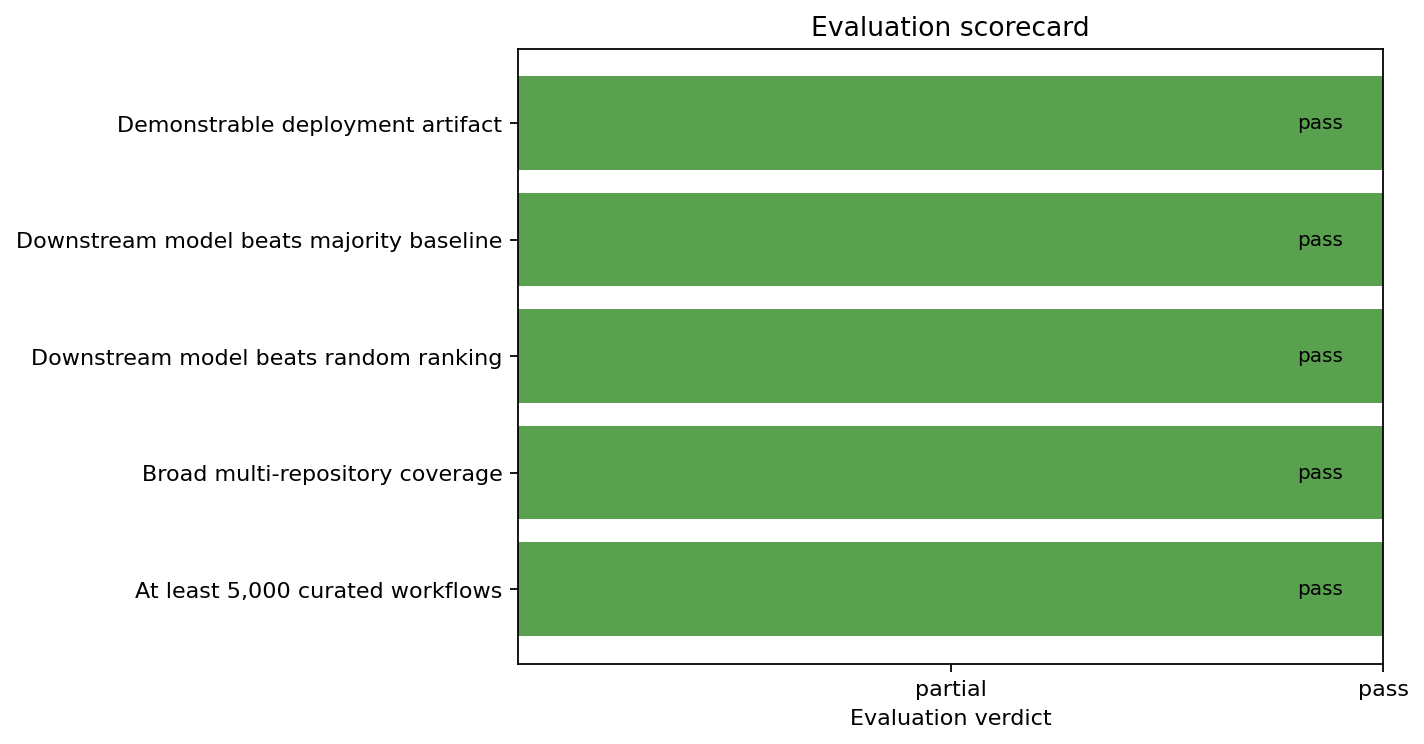
\includegraphics[width=.9\linewidth]{figures/evaluation/evaluation_scorecard.png}
    \caption{Summary of the evaluation criteria.}
\end{figure}

The result answers the business question as a dataset demonstration. It proves that the collected workflows contain learnable signal and can support a realistic downstream task. The test confusion matrix is \([[4,36],[30,911]]\), which shows that the model mainly preserves recall for the dominant concern class. Therefore, the model is best interpreted as a dataset validation baseline and a demo of possible downstream usage.

The most important project findings are not only model metrics. First, public GitHub workflow data is usable at this scale, but quality filtering is necessary because many records lack source patches, source files, or enough discussion. Second, the \texttt{review\_concern} label is highly imbalanced, with about 95.5\% positive labels among labeled rows. Third, PR-AUC is misleadingly high because the positive class dominates; ROC-AUC, macro-F1, balanced accuracy, and class-wise recall are more meaningful. Fourth, capped diff embeddings add signal, but not enough context for robust review-concern detection. This suggests that stronger language-model representations and richer workflow context are required.

\subsection{Review Process}

The CRISP-DM process was followed correctly in structure. Business Understanding defined the dataset product and the downstream \texttt{review\_concern} task. Data Understanding established the scale, repository diversity, field completeness, language distribution, and quality limitations. Data Preparation converted raw nested records into leakage-safe train, validation, and test matrices with repository-level splitting. Modeling compared a majority baseline, logistic regression, and XGBoost variants instead of relying on a single model.

Several choices were appropriate for a first iteration. Removing post-review variables from the feature matrix avoided label leakage. Splitting by repository made evaluation more realistic than random row-level splitting. Comparing tabular-only and embedding-based models made it possible to see that code-diff embeddings help, but only moderately. The Streamlit demo also makes the result inspectable rather than leaving it as a static metric table.

The main weakness is that the evaluation remains offline. There is no manual audit sample yet, no external time-based test set, and no direct feedback from intended users. The current label is also only a proxy for review concern: it captures explicit review activity, not necessarily true software risk. In addition, the enriched GitHub API records were retrieved after merge, so the diff and pull request metadata should be treated as a retrieved PR state rather than a strict opening-time snapshot. The 1,000-token cap also compresses large diffs aggressively, and the model does not reason over repository history or full discussion context. These limitations mean that the project is strong enough as a data mining assignment and dataset demonstrator, but not enough for stronger product claims.

\subsection{Determine Next Steps}

The project should continue through another CRISP-DM iteration rather than stop. The dataset and demo application are ready to present, and the next iteration should focus on improving both data quality evidence and modeling strength.

The highest-priority improvements are to run a manual audit of accepted and rejected samples, collect more negative examples, evaluate on a future time window, tune thresholds for the intended use case, and calibrate predicted probabilities. On the modeling side, the next iteration should try longer-context code models, fine-tuning on review outcomes, richer pull request discussion features, and repository-history features. The goal should be not only to improve ROC-AUC, but also to improve negative-class recall and balanced accuracy.

The recommended decision is therefore: deploy the dataset and Streamlit application as demonstrators, document the model as a baseline, and continue improving the model in the next iteration.
